\subsection{Übersichtszeichnung}

\begin{figure}[h!]
	\centering
	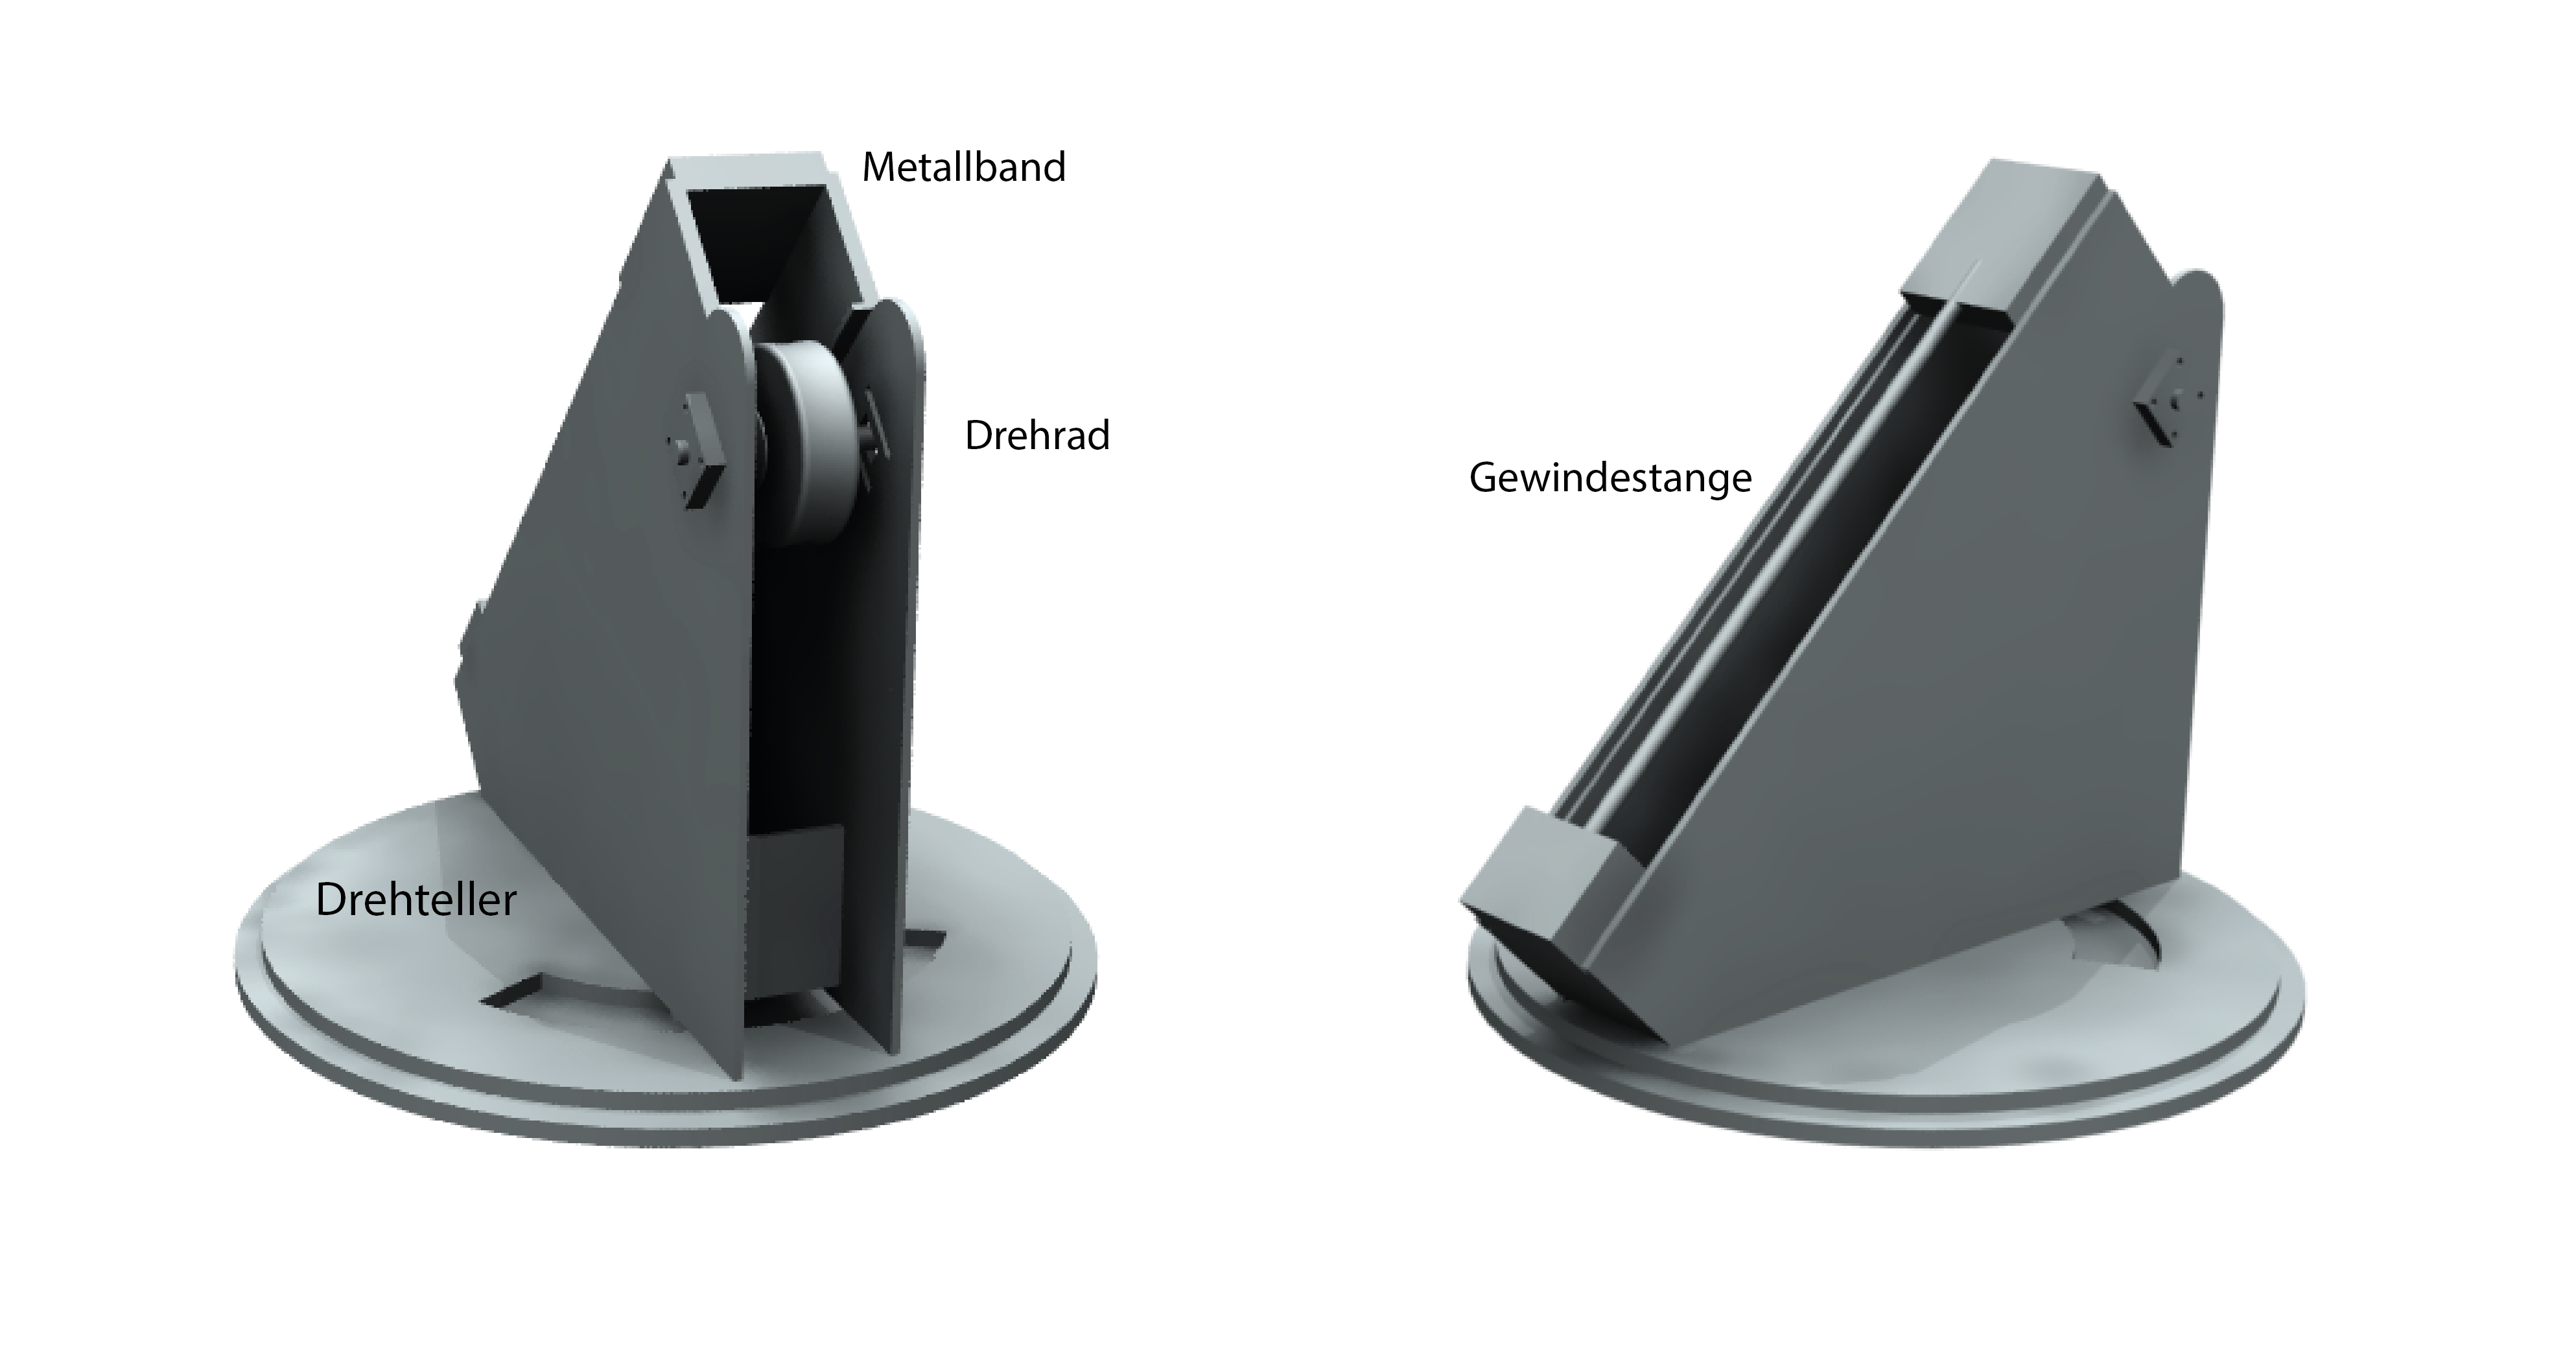
\includegraphics[scale=0.5]{../../fig/StudioLegende.png}
	\caption{Nachlademechanismus}
\end{figure}
Für die Realisierung der Wurfmaschine ist ein Aufbau mittels zwei senkrecht auf einem Drehteller stehenden Hauptplatten aus Holz oder als Variante Kunststoff vorgesehen. Alle Bauteile werden wenn möglich zwischen diesen Hauptplatten untergebracht.
\begin{figure}[h!]
	\centering
	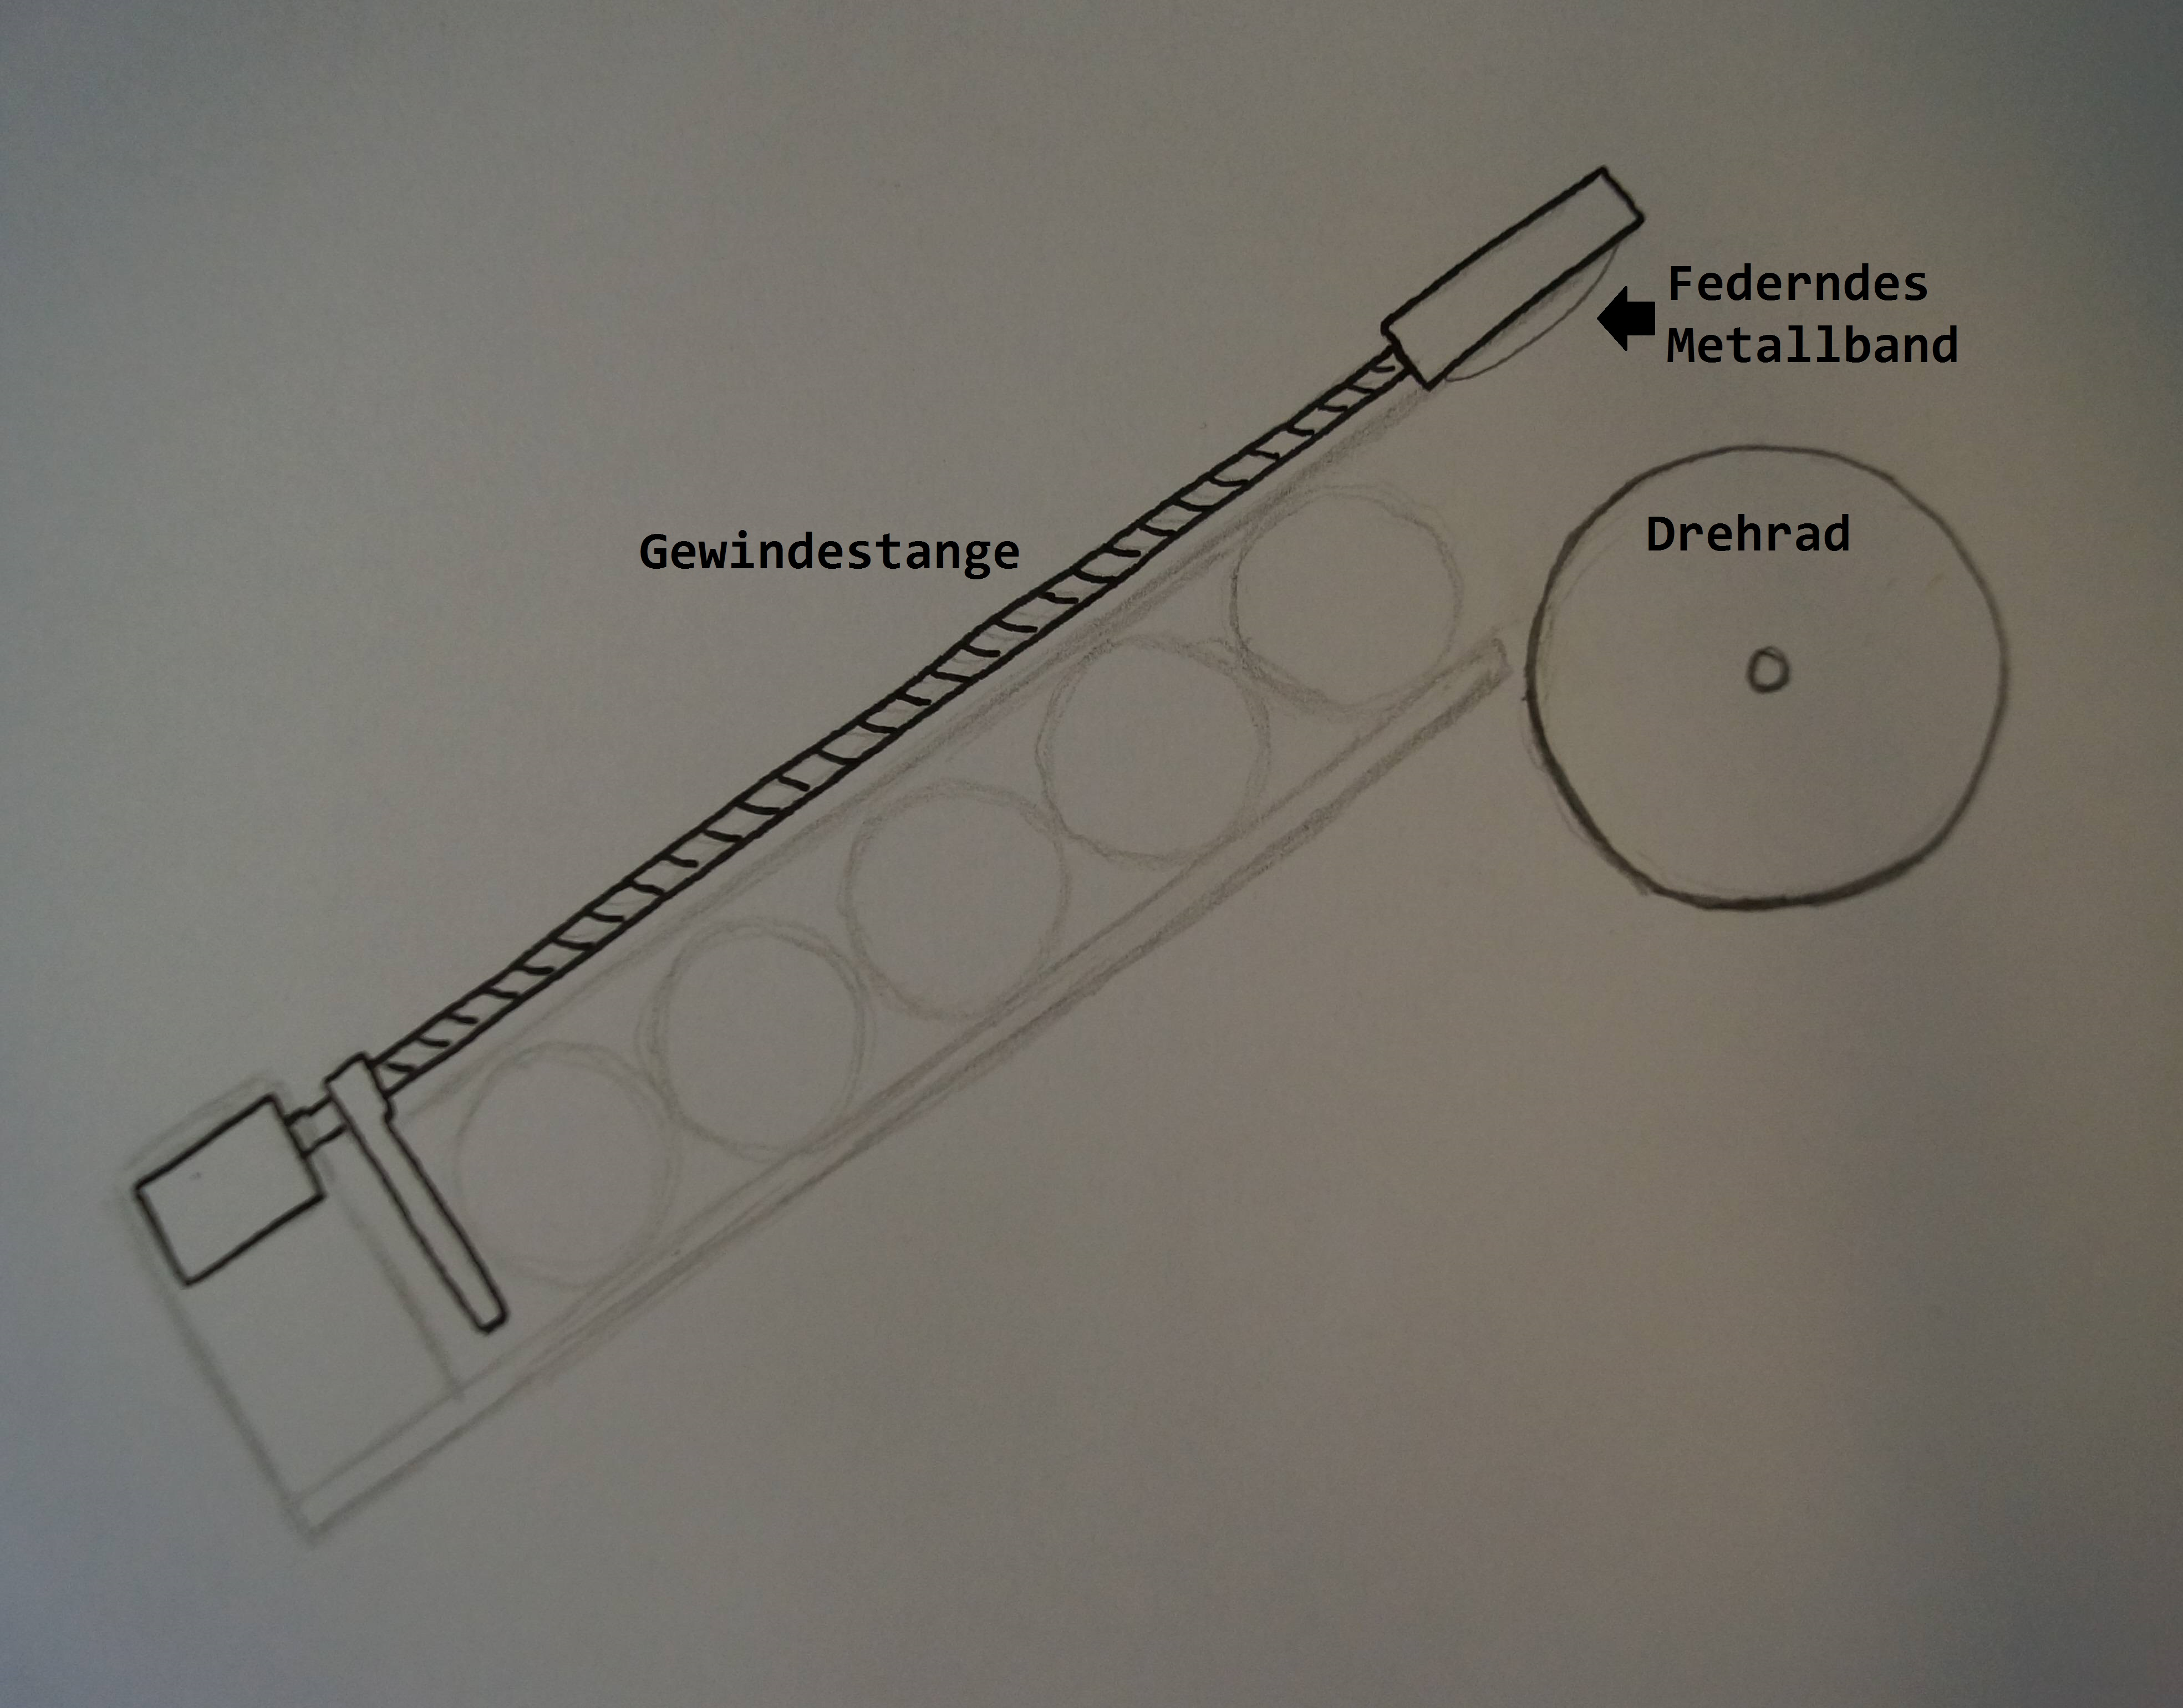
\includegraphics[scale=0.35]{../../fig/Ballnachlader.jpg}
	\caption{Nachlademechanismus}
\end{figure}
Wie in Abbildung 2 zu sehen ist, wird der Ballnachschub mit einer Gewindestange realisiert. Die durch einen direkt angebundenen Motor in Rotation gebrachte Gewindestange, bringt dabei einen Mitnehmer in eine Linearbewegung entlang der Stangenachse und bewegt dadurch die Tennisbälle in Richtung Drehrad.
\begin{figure}[h!]
	\centering
	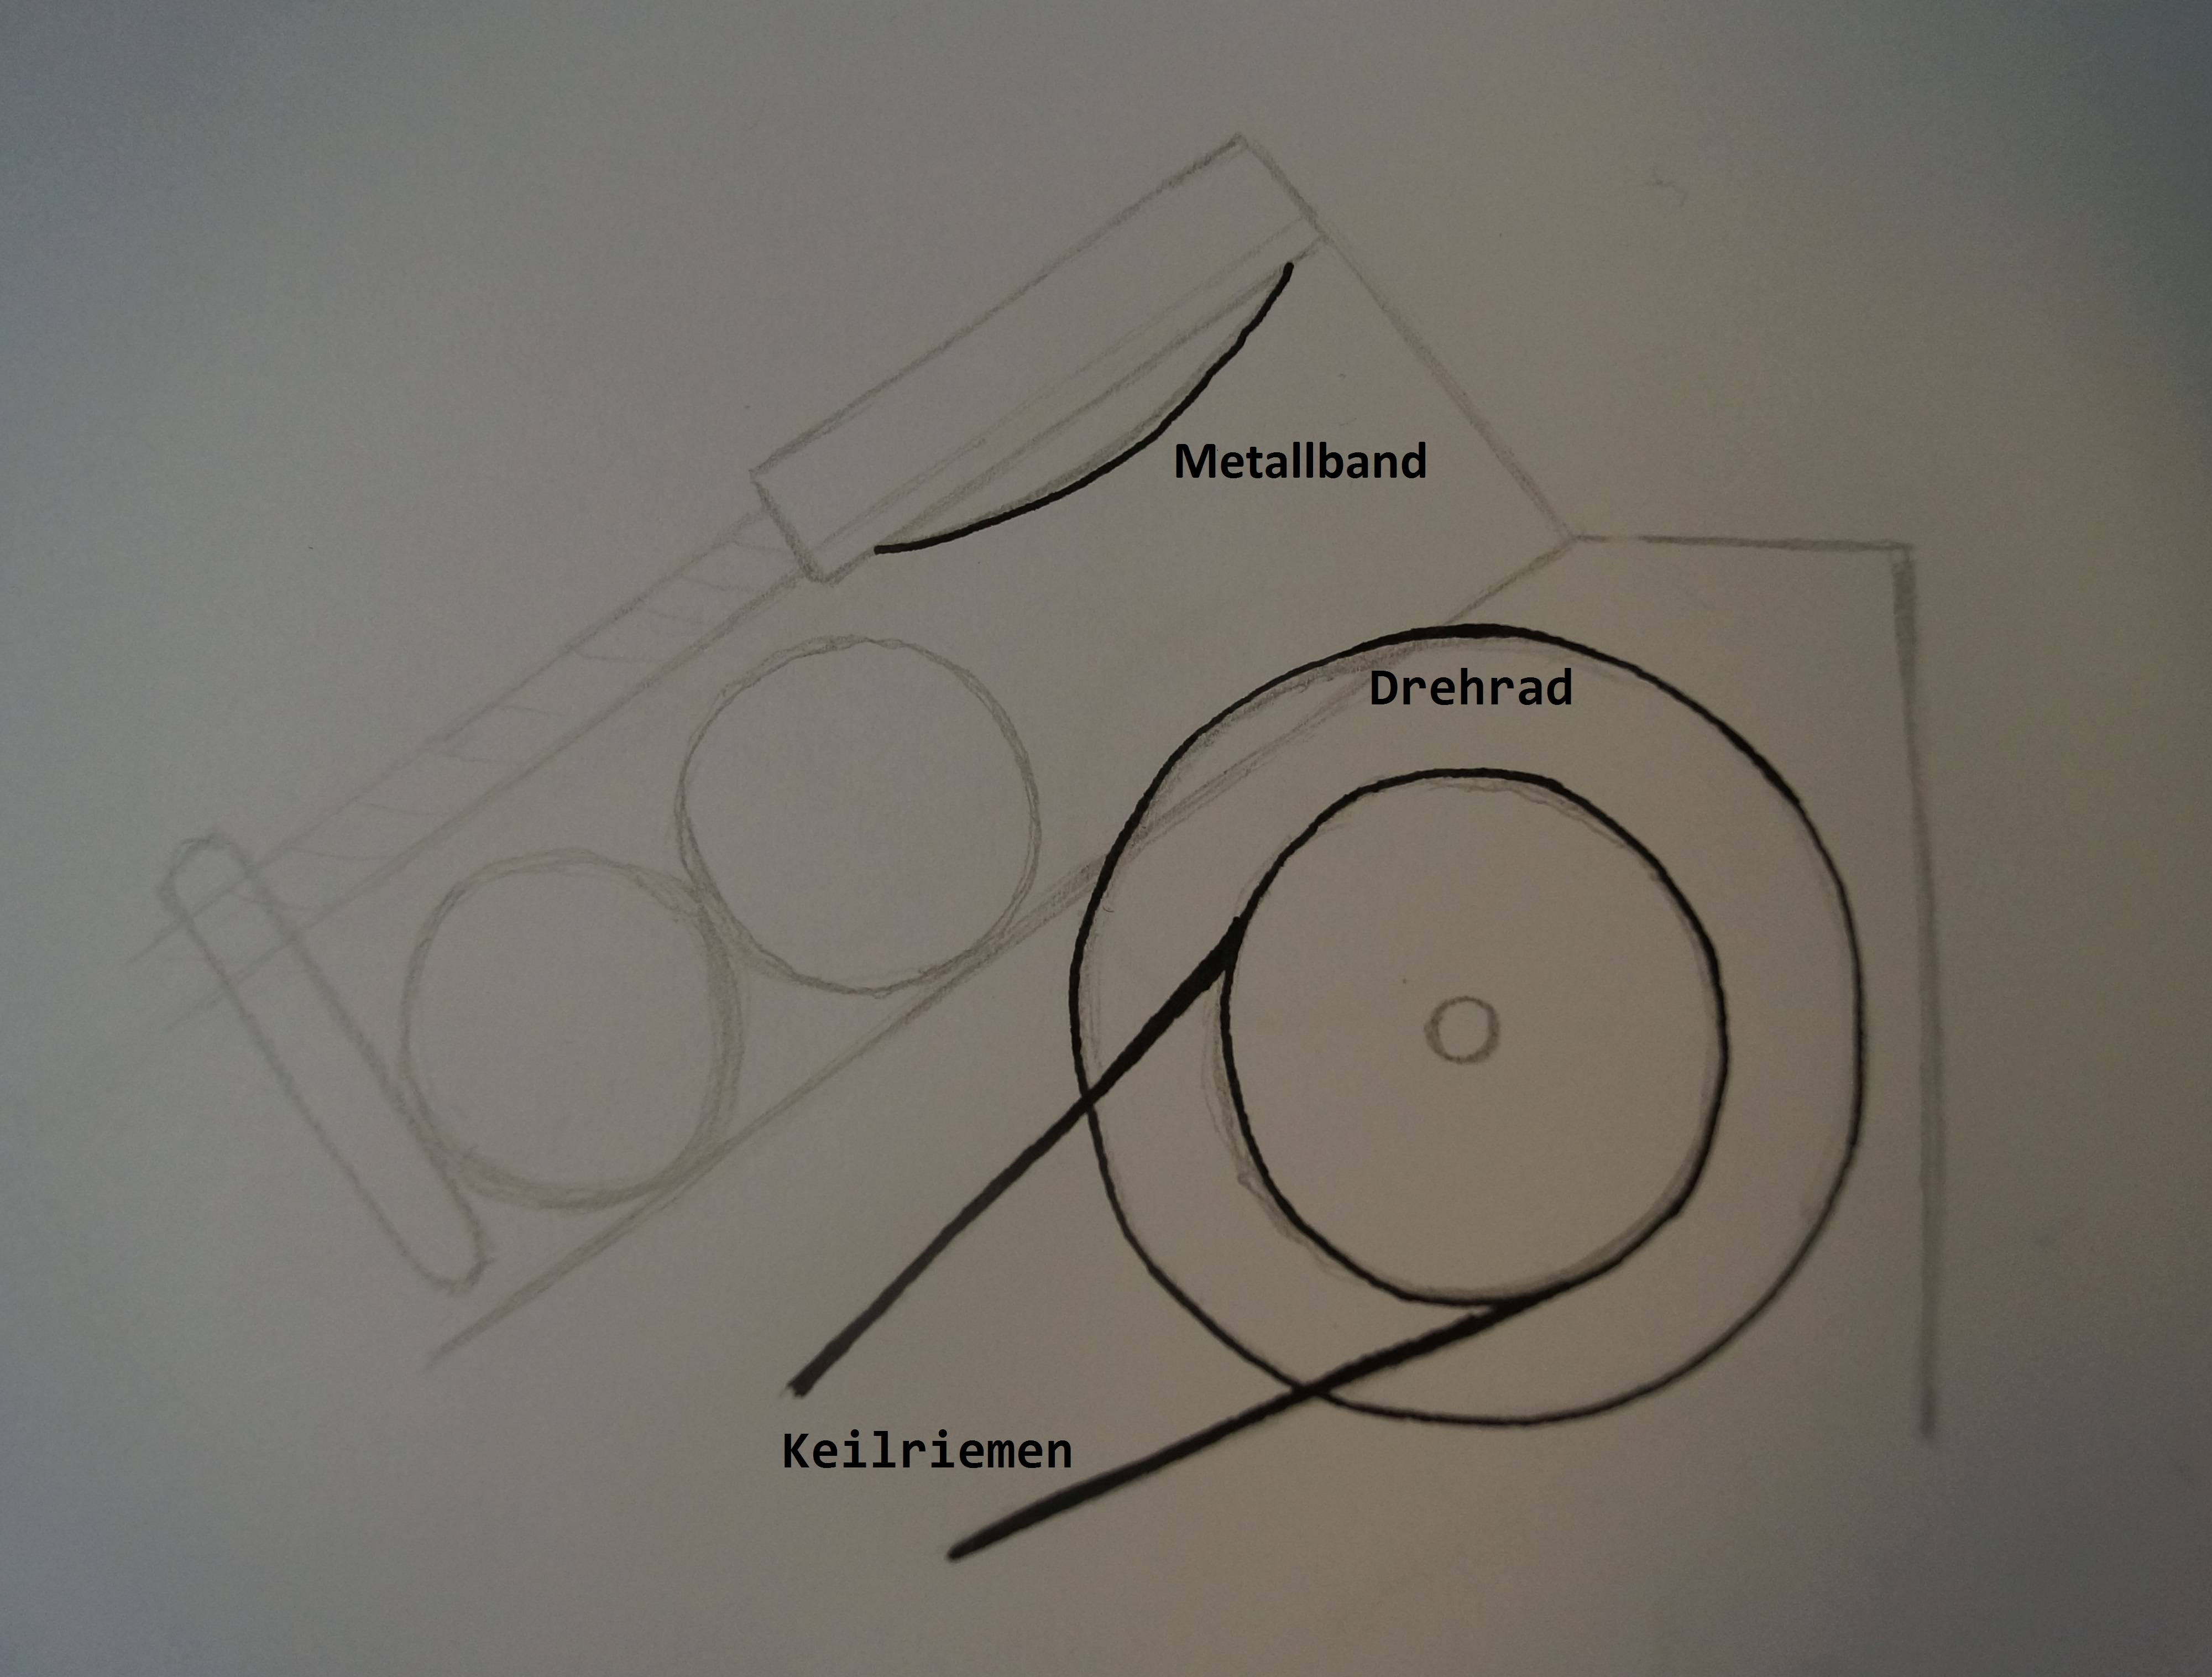
\includegraphics[scale=0.35]{../../fig/Drehrad.jpg}
	\caption{Aufbau des Drehrades}
\end{figure}
Die Bälle werden durch ein rotierendes Drehrad beschleunigt. Das Drehrad wiederum erhält seine Rotation durch einen angebauten Keilriemen, welcher mit einem Motor verbunden ist. Ein über dem Rad angebrachtes Metallband dient, falls nötig, dazu Grössenunterschiede der Bälle zu kompensieren.
\begin{figure}[h!]
	\centering
	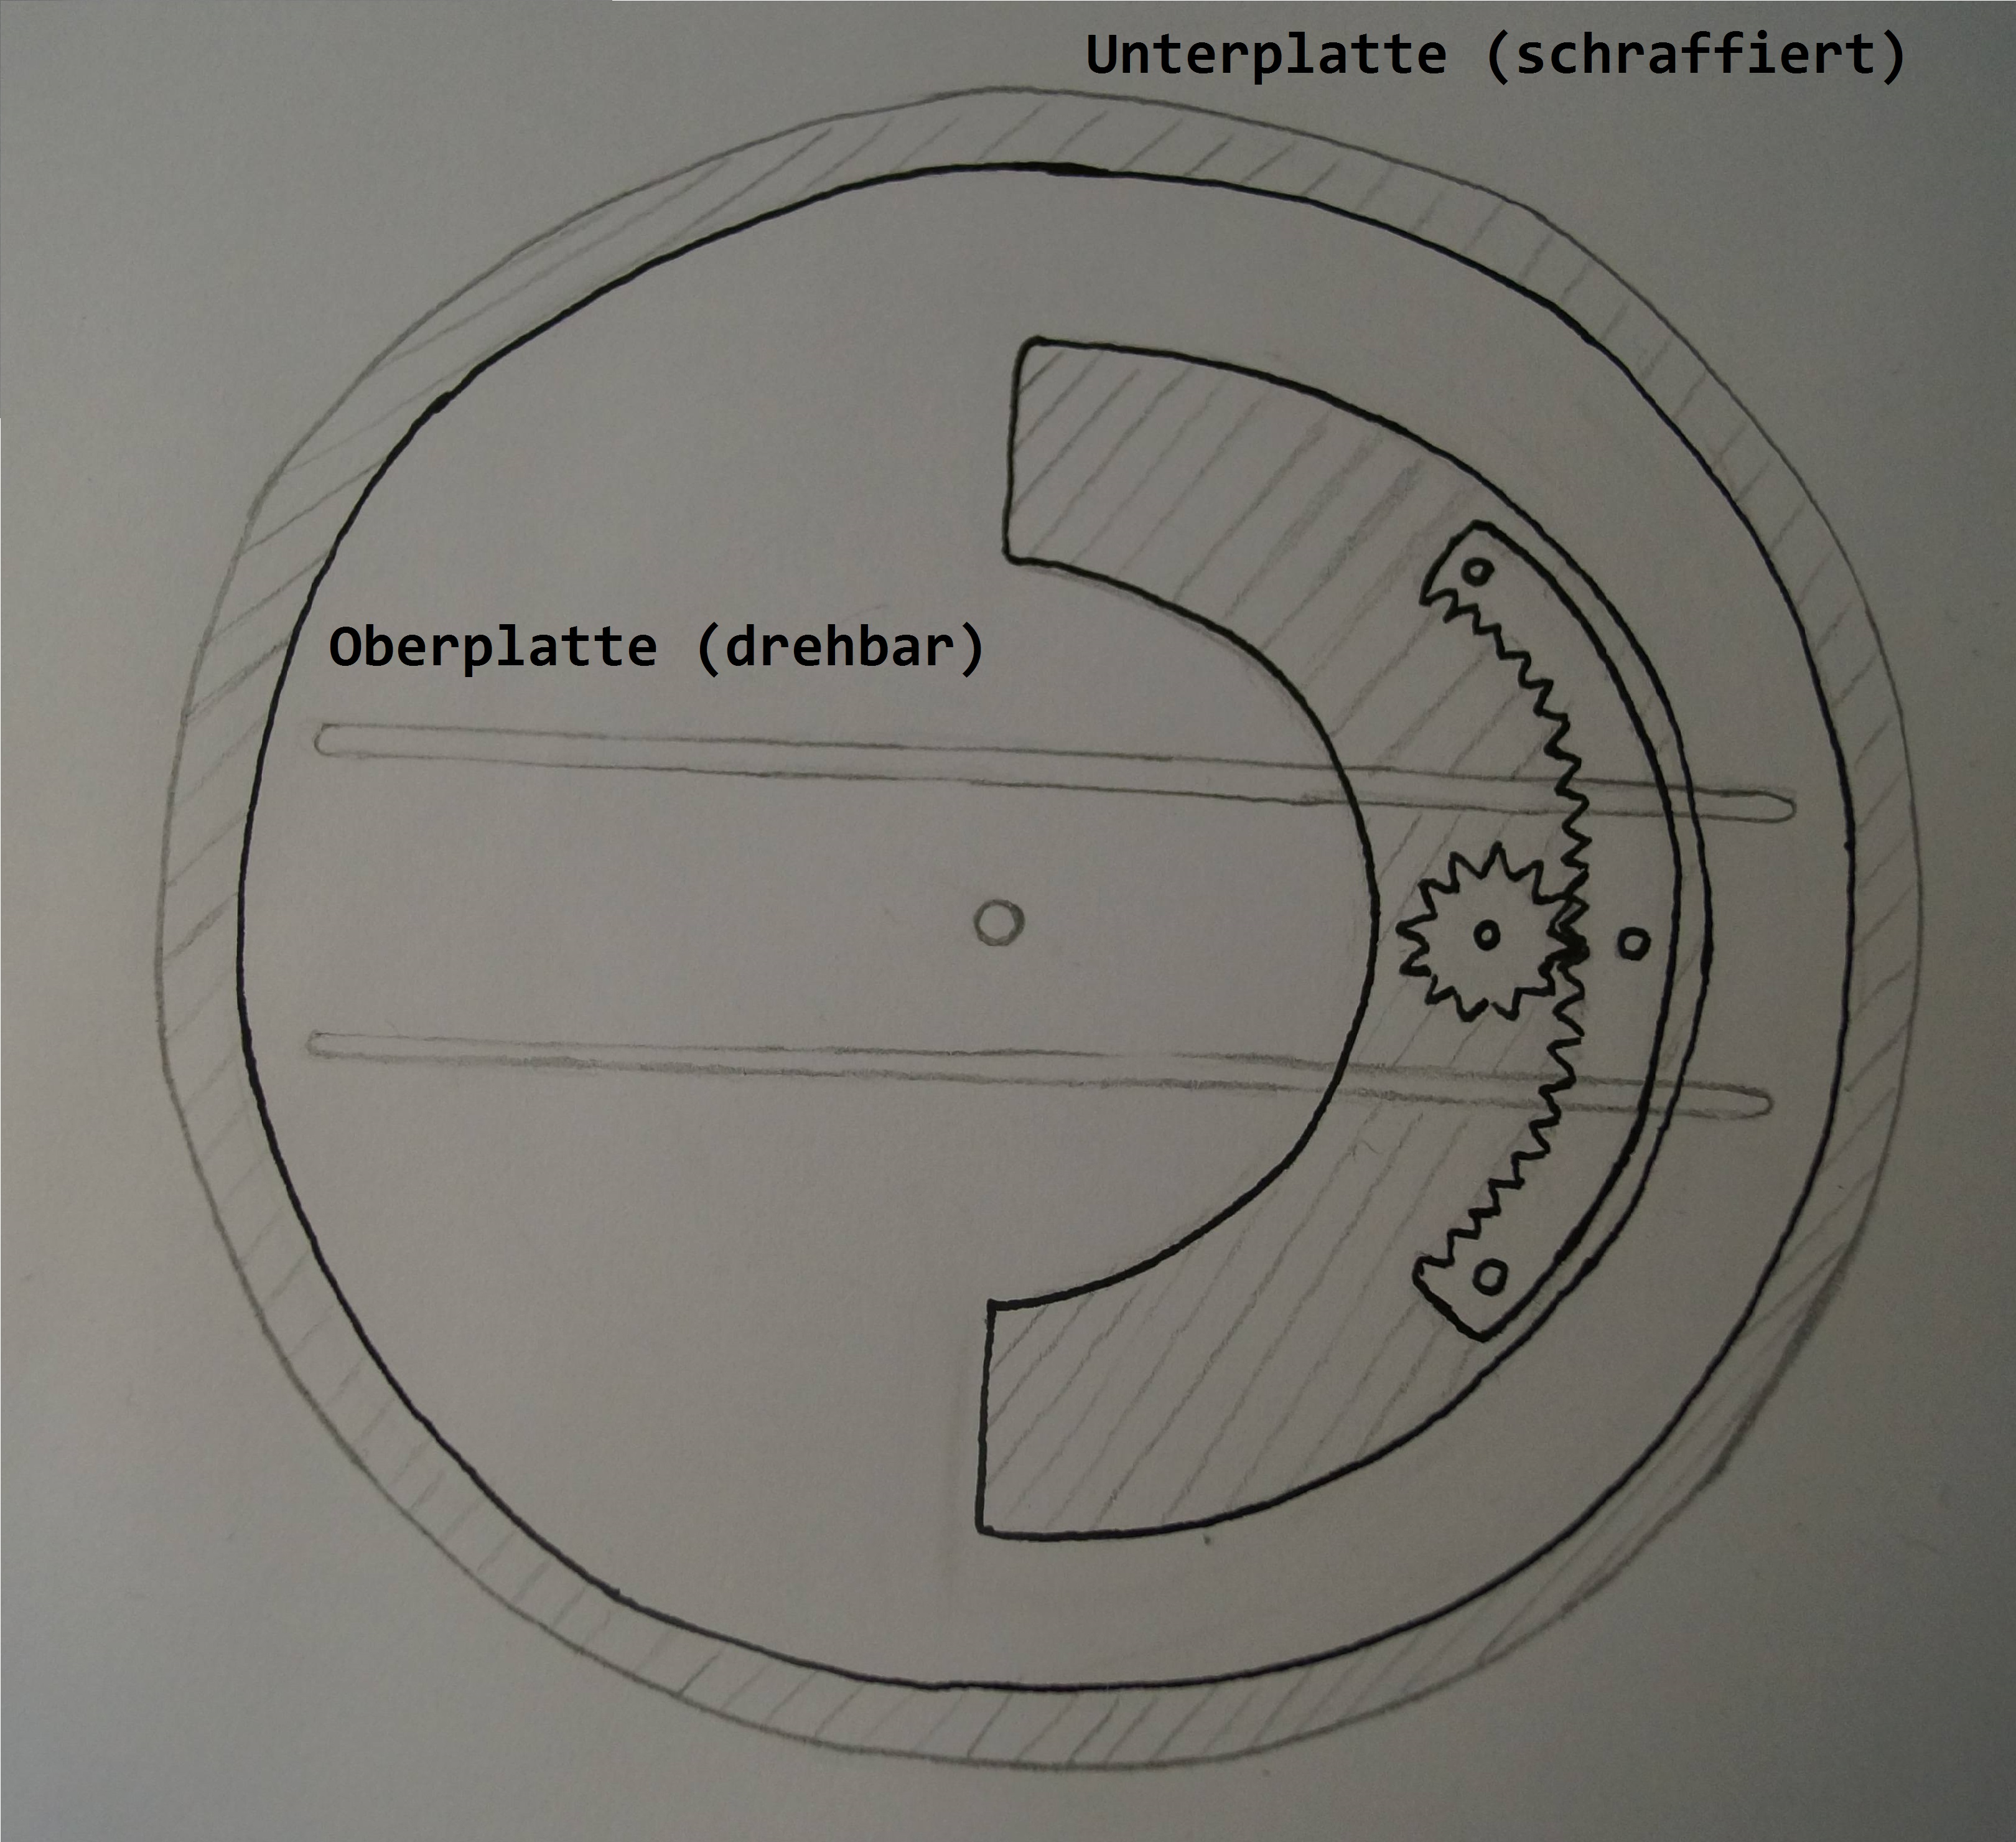
\includegraphics[scale=0.35]{../../fig/Ausrichtvorrichtung_Oben.jpg}
	\caption{Ausrichtvorrichtung von Oben}
\end{figure}
Um die Wurfmaschine horizontal auf den Korb auszurichten, wird die ganze Abschussvorrichtung auf einem Drehteller montiert, welcher auf einer Grundplatte gelagert liegt. An einer auf der Grundplatte befestigten Zahnscheibe, kann nun ein am Drehteller montiertes, angetriebenes Zahnrad, durch Eingriff an der Zahnscheibe, den Drehteller drehen.
\begin{figure}[h!]
	\centering
	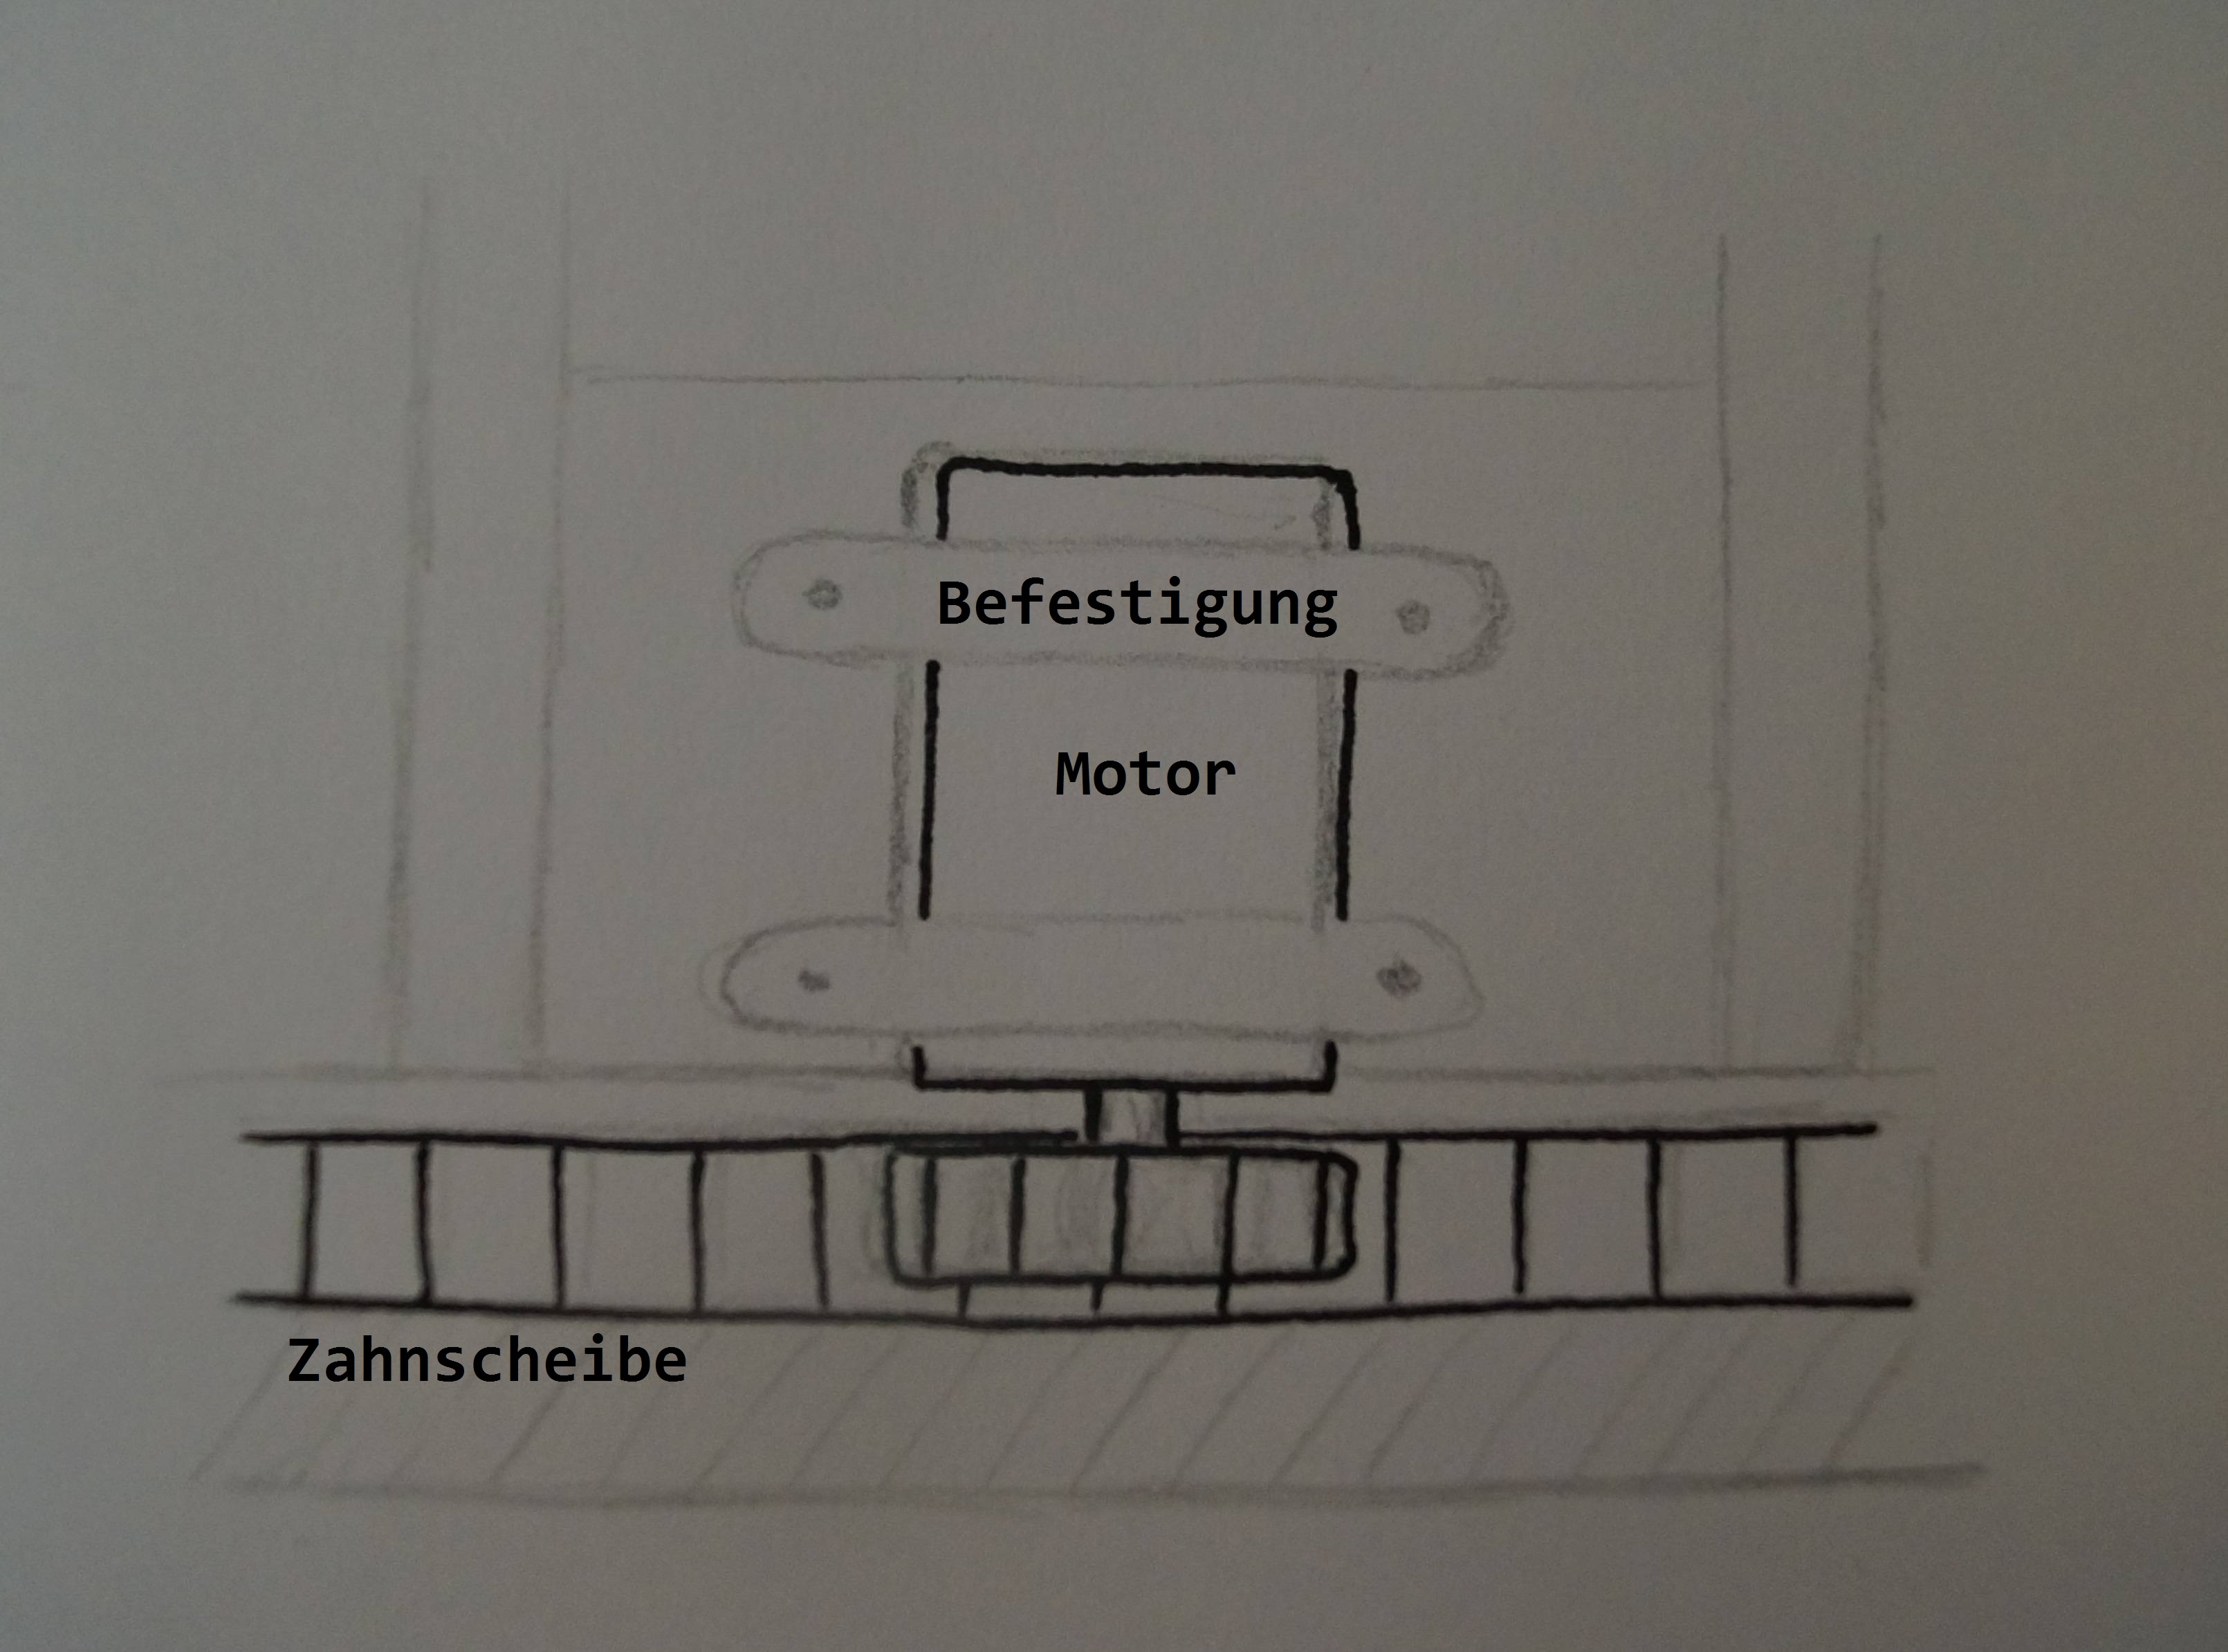
\includegraphics[scale=0.35]{../../fig/Ausrichtvorrichtung_Detail.jpg}
	\caption{Ausrichtvorrichtung im Detail}
\end{figure}
Abbildung 7 zeigt den Zahnradeingriff im Detail von der Seite her.
